% Numbers are macros: CamelCase ones from generated/results.tex (frozen C-v1 run, built by
% reports/mid_submission/build_results.py) and x-prefixed ones from generated/final.tex
% (final-submission analyses and the extension, built by build_final.py).
\begin{abstract}
We test whether the entropy-triggered patch boundaries of the Byte Latent Transformer (BLT) align with syntactic constituent starts in Python, C++ and English, beyond a density-matched null and beyond structure-blind segmenters. On a frozen held-out split of \nTestAll{} files, start F1 exceeds the null in every language (margins \MarginPy{}, \MarginCpp{}, \MarginEn{}; $p\le10^{-4}$), but against the strongest structure-blind baseline BLT \RTwoAll{}: indentation and word-start rules segment better. Three predictions fail as stated, and follow-up tests explain each failure mechanically. The prose margin is largest only because F1 margins scale with target density; relative to the null, code aligns more strongly. The forced-opener reversal (P4) comes from scoring the wrong byte: the start precedes the keyword, while the bytes just after the keyword are segmented below chance. The memory-unsafe residual (O5) exists only after conditioning on identifier entropy, and without that conditioning it is negative. Beyond the proposal, a 14.3M-parameter student distilled from the 99.5M patcher keeps about 90\% of the teacher's held-out margin, and the teacher's alignment peaks at a higher threshold ($\tau^*=\xTauStarTeacherPy$) without overtaking the baselines. Entropy is a genuine but shallow structural signal.
\end{abstract}

\section{Introduction}
Byte-level models remove a fixed subword vocabulary, but they must still decide where to spend computation. BLT groups bytes into variable-length patches whenever a small next-byte model's entropy exceeds a threshold $\tau$ \citep{pagnoni-etal-2025-byte}. If those boundaries fall where syntactic constituents open, the allocation tracks structure. But rare identifiers, word onsets and formatting also raise entropy, so proximity alone cannot separate these explanations.

ESCAPE asks five questions from our proposal. O1/P1: do boundaries align with constituent starts beyond a null that keeps each file's own patch lengths? P2: do they align more at starts than at ends? O2/P3: is code segmented differently from prose? P4: is alignment weaker for constructs whose opener is forced (\texttt{if}, \texttt{for}) than for open-ended ones? O3: does this differ between indentation-based Python and bracket-based C++? O4: does it survive code noise? O5: does extra compute near memory-unsafe C++ survive conditioning on identifier unpredictability? The mid-submission fixed the protocol and reported P1--P4 on the held-out split. This report completes O3--O5, explains the three failed predictions with tests designed for them, checks the statistics against clustering, parser-recovery and context artefacts, and, beyond the proposal, distils the patcher into a 7$\times$ smaller student and evaluates it under the same frozen protocol (\S\ref{sec:ext}).

Our contributions are: (i)~a byte-exact extraction pipeline that restores the reference 512-token sliding window missing from the public conversion; (ii)~a calibration-first protocol with a fixed-EOF density-matched null and structure-blind baselines as the burden of proof; (iii)~held-out results in three languages with every number regenerated from retained per-byte artefacts; and (iv)~mechanistic follow-ups showing that each failed prediction is a statement about which bytes carry entropy, not a failure of measurement.

\section{Background and Related Work}
BLT segments bytes dynamically so that expensive latent computation operates over patches \citep{pagnoni-etal-2025-byte}. We analyse its entropy patcher, not downstream accuracy. BPE fixes its merge table in advance and spends the same units on boilerplate as on logic \citep{sennrich-etal-2016-neural}. ByT5 and CANINE remove the vocabulary but process every byte or character uniformly \citep{xue-etal-2022-byt5,clark-etal-2022-canine}. BLT is the first model at scale whose segmentation is both byte-level and decided at inference time, so each boundary is a claim the model makes and can be checked against external structure. Structural probes recover syntax from trained representations \citep{hewitt-manning-2019-structural,feng-etal-2020-codebert}, but they need a trained probe or code-specific objectives. We ask instead whether an unsupervised compression signal with no parser in the loop recovers constituents as a side effect. Statistical word segmentation has long placed boundaries by predictability \citep{brent1999segmentation,goldwater2009word}, and it was always checked against observable word boundaries. We apply the same check to the patcher, with tree-sitter ASTs for code and benepar parses \citep{kitaev-klein-2018-constituency} for English. For the extension we use online knowledge distillation \citep{hinton2015distilling}.

\section{Protocol}
\label{sec:protocol}
\paragraph{Data and checkpoint.} The frozen manifest has \nSamples{} samples: 8{,}000 Python functions from CodeSearchNet \citep{husain2019codesearchnet}, 8{,}000 C++ files from The Stack \citep{kocetkov2022stack} and 300 WikiText-103 paragraphs \citep{merity2017pointer}, all restored and hash-verified. We load the 99.5M-parameter patcher of \texttt{itazap/blt-1b-hf} (revision \texttt{91aa6b8e}) in float32 with $\tau=1.3354$ nats, no length cap, and the reference 512-token sliding window in 8{,}192-token chunks. Six of eight fidelity gates passed as declared; two criteria (tokenizer EOS, random-byte density) were amended, and the amended set \FidelityAda{} on the cluster stack (Appendix~\ref{app:fidelity}). In October the corpus and teacher artefacts on the cluster were deleted and then regenerated. The regenerated run reproduced the frozen per-file, score and diagnostic files byte for byte.

\paragraph{Metric, null and baselines.} Entropy at byte $i$ is $H_i=-\sum_v p_\theta(v\mid x_{<i})\log p_\theta(v\mid x_{<i})$ over 260 symbols. Predictions are interior entropy boundaries. Targets are the unique starts of non-wrapper constituents (outermost node wins ties), excluding byte 0 and file end. Maximum-cardinality one-to-one matching within $k$ bytes gives pooled P, R and F1. Each language is split 20/80 by seeded SHA256 rank into calibration and test files, and only calibration files choose $k\in\{0,1,2,4,8\}$, by the median per-file F1 margin over the null; $k=0$ was selected everywhere. The null shuffles each file's (length, reason) patch pairs except the last, which stays fixed so that file end is never a boundary, and so it preserves the patch-length multiset and boundary count. We use \nPerm{} seeded permutations per file and \nBoot{} paired file-bootstrap replicates. A structural reading must also beat boundaries at every newline, at indentation changes, and at every word start under the same targets and matching.

\section{Results on the Proposal's Objectives}
\TableMain
\paragraph{P1 and the structure-blind burden.} Start F1 exceeds the null in every language (Table~\ref{tab:main}), with ratios of 4--5$\times$ in code. Against the strongest structure-blind baseline, however, BLT \RTwoAll{} (Table~\ref{tab:baselines}): Python \VsBasePy{} \VsBaseCIPy{} against indentation, C++ \VsBaseCpp{} against word starts, and English \VsBaseEn{} against word starts. The margin is positive across languages, but its magnitude depends on target density. Most of what it tracks is still line and word segmentation.

\paragraph{Precision versus recall.} The proposal's mechanism predicted precision above recall: cheap interiors and forced closing delimiters would rarely trigger, so boundaries would be few and well placed. Instead precision \PrecRecAll{} (Python \PrecPy{}/\RecPy{}; C++ \PrecCpp{}/\RecCpp{}; English \PrecEn{}/\RecEn{}). The asymmetry follows from the trigger rule. Since $H\le\log B$, every boundary sits where at least $e^{\tau}\approx3.8$ continuations were live. Identifier interiors, strings and comments are flat without being syntactic, so predictions outnumber targets roughly ten to one, which caps precision while the same density guarantees high recall. P2 holds in the predicted direction: end margins are negative (\EndMarginPy{}, \EndMarginCpp{}, \EndMarginEn{}), so closing delimiters are anti-aligned.
\TableBaselines

\paragraph{Why P3 came out reversed.} The proposal predicted large BPP variance in code and near-chance alignment in prose. The first half holds: within-file BPP variance is \BppVarCpp{} in C++ and \BppVarPy{} in Python against \BppVarEn{} in English, because boilerplate stretches alternate with dense logic. The second half fails: the prose margin \MarginProse{} exceeds the code margin \MarginCode{}. Two facts explain this. First, a benepar constituent always begins at a word, and the patcher fires at word onsets, so the word-start rule alone reaches F1 \StrongestFoneEn{} in English. Prose ``alignment'' is word segmentation measured against a parse. Second, F1 margins are not comparable across target densities. English has far more targets per prediction, which raises both observed and null F1. On the scale-free ratio to the null, code aligns \emph{more} strongly than prose (\xRatioPy{}$\times$ Python, \xRatioCpp{}$\times$ C++, \xRatioEn{}$\times$ English, file-bootstrap intervals in Appendix~\ref{app:extra}). The reversal therefore says that the absolute margin depends on target density, not that prose carries more structure.

\TableTypes
\paragraph{Why P4 came out reversed, and what the forced bytes do.} By type, forced openers have larger start-recall margins than open-ended constructs (Table~\ref{tab:types}; mean \DetMarginPy{} vs.\ \OpenMarginPy{} in Python, \DetMarginCpp{} vs.\ \OpenMarginCpp{} in C++), the opposite of P4. The mid-report's conjecture was that a start boundary sits \emph{before} the keyword, where the choice of statement is still open, while the forcing predicted by the proposal applies to the bytes after it. We tested this directly. For every primary target start $s$ we take its first token (the identifier run at $s$: the keyword for forced openers) and score the boundary rate at fixed positions against the same \nPerm{} null draws as the frozen scorer, so the start rows \xPosCheck{} the frozen type recalls exactly (Table~\ref{tab:p4pos}). The rest of the keyword is segmented below chance (Python \xKwDetPy{}, C++ \xKwDetCpp{}), and the byte right after it almost never starts a patch (rate \xPostKwRateDetPy{} and \xPostKwRateDetCpp{} against null rates of \xOffNullPy{} and \xOffNullCpp{}). For open-ended constructs the byte after the first token stays near the null (\xPostKwOpenPy{}, \xPostKwOpenCpp{}). The boundary reappears where choice reopens. In Python the next non-space byte begins the condition, and its boundary rate is \xNextRateDetPy{} (\xNextDetPy{}). In C++ that byte is the equally forced \texttt{(} (\xNextIfCpp{} after \texttt{if}), and the boundary moves one byte further, to the condition, at offset four (rate \xOffDetCppIV{}; Figure~\ref{fig:offsets}). \texttt{return}, which the taxonomy classes as open-ended, behaves the same way after its keyword (\xPostKwReturnPy{}, \xPostKwReturnCpp{}). P4's mechanism therefore holds at the bytes it is about: once a keyword is committed, its continuation is predictable and is segmented far below chance. A start-offset metric cannot see this, because the start byte is exactly where the forcing has not yet happened.
\xTableFour

\begin{figure*}[t]
\centering
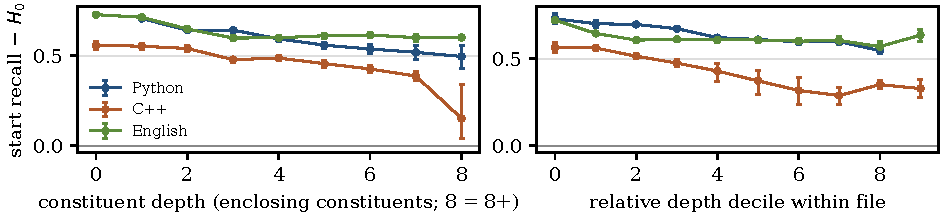
\includegraphics[width=\textwidth]{generated/depth_normalised.pdf}
\caption{O3: held-out start recall minus mean $H_0$ recall by scaffold-free depth. Left: the number of enclosing constituents (raw tree-sitter depth also counts grammar scaffolding such as \texttt{block}, \texttt{compound\_statement} and \texttt{argument\_list}, whose amount differs by language). Right: within-file relative depth decile. Strata with at least 200 starts; 10{,}000 frozen null draws; file-bootstrap 95\% intervals.}
\label{fig:depth}
\end{figure*}
\paragraph{O3: Python versus C++ on a common depth scale.} Raw tree-sitter depth is not comparable across languages: C++ statements sit under more scaffolding nodes than Python ones, and benepar trees are collapsed differently again. We therefore count depth in constituents, as the number of stored target-type nodes that strictly enclose a node, and also normalise it within each file (Figure~\ref{fig:depth}). On this common scale all three languages align most at the outermost constituents. From one enclosing constituent to seven, the margin falls from \xDepthOnePy{} to \xDepthSevenPy{} in Python, from \xDepthOneCpp{} to \xDepthSevenCpp{} in C++, and from \xDepthOneEn{} to \xDepthSevenEn{} in English. Python exceeds C++ at every depth both languages share and at every relative-depth decile. English is nearly flat below the top levels, consistent with word-onset alignment holding at every level of a parse. The indentation-versus-brackets contrast that O3 asked about shows up in the baselines rather than in the depth profile. In Python the indentation rule is the strongest baseline, because indentation \emph{is} the grammar. In C++ word starts are the strongest baseline, and BLT's deficit to them (\VsBaseCpp{}) is smaller than its deficit to indentation in Python (\VsBasePy{}).

\paragraph{O4: robustness to noise, by rate.} At the frozen rates (\OFourRate{} of lines or keywords, \OFourCaseRate{} of identifiers) every noised margin stays at or above \OFourMinMarginPy{} (Python) and \OFourMinMarginCpp{} (C++), and the largest drop is \OFourWorstDmPy{} for \OFourWorstPy{} noise in Python (Appendix Table~\ref{tab:o4}). To test whether this ``graceful degradation'' depends on the rate, we rebuilt the same \xOFourSweepFiles{} files per language with each noise type at 5, 10, 20 and 40\% (case inversion at 25, 50 and 100\%), and scored them with the unchanged O4 scorer (Figure~\ref{fig:o4}). Only indentation noise does damage that grows steadily with rate, roughly in proportion to the share of lines touched: from \xOFourIndentLoPy{} at 5\% to \xOFourIndentHiPy{} at 40\% in Python, and from \xOFourIndentLoCpp{} to \xOFourIndentHiCpp{} in C++. This is the expected signature of a patcher whose statement boundaries ride on line layout. Keyword typos barely move alignment (\xOFourTypoHiPy{} and \xOFourTypoHiCpp{} at 40\%). They do lower bytes per patch in proportion to rate (\xOFourTypoBppPy{} and \xOFourTypoBppCpp{} at 40\%), because a misspelt keyword is unpredictable and is split into more patches. Renaming identifiers costs at most \xOFourCaseMaxPy{} (Python) and \xOFourCaseMaxCpp{} (C++), with no trend between 25\% and 100\% of names, consistent with identifiers already being near-arbitrary for the patcher. Every noised margin stays at or above \xOFourSweepMinMargin{}.
\begin{figure*}[t]
\centering
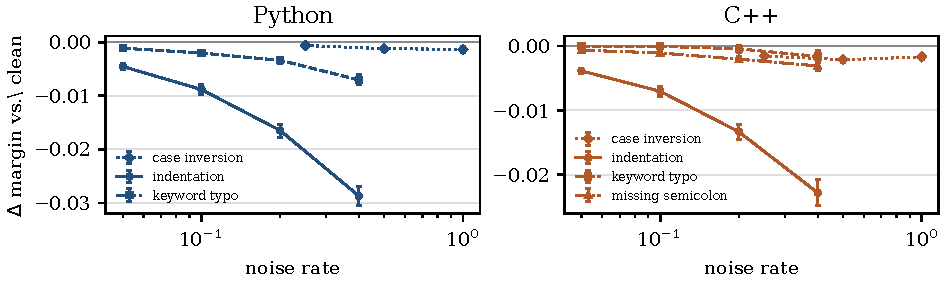
\includegraphics[width=\textwidth]{generated/o4_sweep.pdf}
\caption{O4 rate sweep: change in the start margin over $H_0$ relative to the clean files, by noise type and rate (log scale), on the same held-out files. Targets are clean constituents mapped to noised offsets; 1{,}000 permutations per file; paired file-bootstrap 95\% intervals.}
\label{fig:o4}
\end{figure*}

\paragraph{O5: is there a semantic residual near memory-unsafe code?} We first audited the region labels (\texttt{docs/O5\_LABEL\_AUDIT.md}). Re-running the tree-sitter queries reproduced \xAuditRepro{} frozen regions exactly, and an independent lexical labeller agreed on every label for \xAuditAgree{} audited statements. The two disagreements were address-of operations inside casts, which tree-sitter labels correctly. The frozen regression gives unsafe statements \xOFiveFull{} \xOFiveFullCI{} extra boundaries per byte after file fixed effects and identifier controls. Refitting it as a nested sequence (our refit \xOFiveCheck{} the frozen coefficients) changes the reading (Table~\ref{tab:o5}). With file fixed effects only, unsafe statements receive \emph{fewer} boundaries (\xOFiveRaw{} \xOFiveRawCI{}), because they use more predictable identifiers. The positive coefficient appears only after conditioning on identifier entropy, and identifier share alone does not flip it. The conditional effect is \xOFiveRel{} of the comparison statements' mean density, and \xOFiveVsIdent{} of the effect of one standard deviation of identifier entropy. It is most plausibly carried by the unsafe operator bytes themselves (\texttt{*}, \texttt{\&}, \texttt{new}), which are surface tokens. O5 therefore finds no evidence that the patcher allocates extra compute to memory risk. What survives the confound is a small conditional surface effect, and the unconditional effect points the other way.
\xTableOFive

\paragraph{Are the intervals too narrow?} The 8{,}000 Python functions come from only \xRepoN{} repositories. Resampling repositories instead of files widens the Python interval \xRepoWiden{}$\times$ to \xRepoCI{}, which still excludes zero. Tree-sitter error recovery affects \xErrShare{} of C++ test files, and their margin differs from clean parses by \xErrDiff{} \xErrDiffCI{}. Files longer than 8{,}191 bytes, whose context resets at chunk edges, make up \xLongShare{} of C++ test files but \xLongBytes{} of its bytes, and their margin differs by \xLongDiff{} \xLongDiffCI{}. Every subset's margin is recomputed exactly from the frozen per-file counts (Appendix Table~\ref{tab:robust}). Under $k=1$ and $k=2$ as test-split sensitivity checks the margins shrink, as the calibration curve predicts (Appendix Table~\ref{tab:k}), and BLT never overtakes the strongest baseline.

\section{Beyond the Proposal: a Distilled Patcher}
\label{sec:ext}
The proposal needed no training. We added one experiment, labelled here as an extension and separately pre-registered: can a much smaller byte model reproduce the patcher's boundaries, and does structural alignment survive distillation? A 14.3M-parameter student (384 dimensions, 8 layers, 6 heads, BLT-style byte transformer) was trained from scratch by online distillation, $\alpha\,\mathrm{CE}+(1-\alpha)T^2\,\mathrm{KL}(p_T\Vert p_S)$ with $\alpha=0.1$ and $T=2$, on $\le$512-byte windows of a disjoint extension corpus. That corpus has 29{,}000 files: CodeSearchNet functions from repositories not in the evaluation set, WikiText paragraphs from unused articles, and Stack C++ from other repositories, split by repository or article. On held-out extension windows the student's boundaries reach F1 \xDistFone{} against the teacher's. Dropping the teacher ($\alpha=1$, same data, seed and schedule) reaches \xAlphaFone{}, and placing a boundary at every word start reaches \xWordVsTeacherFone{} (Appendix Table~\ref{tab:alpha}). The $\alpha=1$ student predicts the true next byte better (\xAlphaBpb{} vs.\ \xDistBpb{} bits/byte; teacher \xTeacherBpb{}), so distillation trades a little compression for agreement with the teacher's segmentation.

\paragraph{Held-out alignment.} We extracted the student on all 16{,}300 corpus files with stride-1 fresh 512-byte windows, the regime it was trained in. Before that, the extractor had to reproduce the committed golden-fixture scores on the cluster GPU, and it did so exactly (largest F1 deviation \xGateMaxDev{}). The student then went through the frozen C-v1 pipeline with its own calibration record, which again selected $k=0$ everywhere (Table~\ref{tab:student}). It keeps \xStuRetainPy{}, \xStuRetainCpp{} and \xStuRetainEn{} of the teacher's margin (Python, C++, English). The paired deficits are small but resolved (\xStuDiffPy{} \xStuDiffCIPy{} in Python), and the student, like the teacher, stays below the structure-blind baselines. The student fires more often (mean BPP \xStuBppPy{} vs.\ \xTeaBppPy{} in Python), which buys recall at the cost of precision. A control on 300 test files per code language restricts the \emph{teacher} to the student's fresh 512-byte windows. This costs \xTfiveDiffPy{} \xTfiveDiffCIPy{} (Python) and \xTfiveDiffCpp{} \xTfiveDiffCICpp{} (C++) of F1, about \xTfiveSharePy{} and \xTfiveShareCpp{} of the student's deficit on the same files (Appendix Table~\ref{tab:t512}). The 512-byte context explains part of the gap, and model capacity the rest.
\xTableStudent

\paragraph{Threshold and tolerance.} The checkpoint's $\tau$ was set for compression, not alignment. We swept $\tau\in\{0.8,1.0,1.335,1.7,2.0,2.5\}$ on calibration files only and pre-registered $\tau^*$ as the argmax of the median per-file margin, with ties going to the smaller $\tau$. Two readings of the criterion (per-file and pooled null means) agreed. For the teacher $\tau^*=\xTauStarTeacherPy{}$ in all three languages (calibration gain \xTauGainTeacherPy{} in Python), and for the student $\tau^*=\xTauStarStudentPy{}$ (Python), \xTauStarStudentCpp{} (C++) and \xTauStarStudentEn{} (English) (Appendix Figure~\ref{fig:tau}). The student's English optimum sits at the edge of the grid, where its entropy runs higher than the teacher's. The pre-registered grid was not extended after seeing this, so each language with its own $\tau^*$ was confirmed in a separate run. After re-freezing $k$ under $\tau^*$, each model's test split was scored exactly once (Table~\ref{tab:tau}): the teacher's margin rises to \xTauConfTeacherPy{} (Python), \xTauConfTeacherCpp{} (C++) and \xTauConfTeacherEn{} (English), a paired gain of \xTauPairGainTeacherPy{} \xTauPairGainCITeacherPy{} in Python, and it remains below the strongest baseline (\xTauConfVsBaseTeacherPy{}, \xTauConfVsBaseTeacherCpp{}, \xTauConfVsBaseTeacherEn{}). The student's margin at its own $\tau^*$ is \xTauConfStudentPy{}, \xTauConfStudentCpp{} and \xTauConfStudentEn{}, also below the baselines. Fewer, higher-entropy boundaries are better aligned, but no threshold turns entropy into a parser.
\xTableTau

\paragraph{The confirmatory English test.} The 300 evaluation paragraphs were inspected during exploratory analysis before the protocol was frozen. We therefore pre-registered a holdout of the 120 lowest-ranked WikiText articles that neither evaluation nor distillation used, \xHoldFiles{} paragraphs with benepar structure, and scored it once after team sign-off (Table~\ref{tab:holdout}). The teacher's margin is \xHoldTeaMargin{}, against \MarginEn{} on the evaluation paragraphs, and the student's is \xHoldStuMargin{}. Both stay below word starts (\xHoldTeaVsWord{} and \xHoldStuVsWord{}), so the English findings replicate on untouched text.
\xTableHoldout

\paragraph{Cost.} On one \xEffGpu{} the student's forward pass is \xEffForward{}$\times$ faster than the teacher's at the same input (Appendix Table~\ref{tab:eff}), and \xEffRolling{}$\times$ faster under the rolling extractor used for both student runs. The native teacher processes a file in a single sliding-window pass at \xEffNative{} tokens/s. The student architecture does not implement that pass, which is why its full-corpus extraction took about 20 GPU-hours per shard. A deployment-grade student would need the same single-pass kernel.

\paragraph{Byte balancing and domain adaptation.} Two follow-ups ran after the main analysis, on the pre-registered 600-file code subset of Table~\ref{tab:t512} plus the English test split (Appendix Table~\ref{tab:arms}). Full-corpus extraction of these models did not fit before the deadline, so both are exploratory. C++ is 73\% of the distillation bytes. A student trained with every domain drawn to an equal expected byte share, and otherwise identical, agrees with the teacher's boundaries on held-out windows at F1 \xBalWinFone{} (distilled student: \xBalRefWinFone{}), and its margin differs from the distilled student's by \xBalDiffPy{} \mbox{\xBalDiffCIPy{}} (Python), \xBalDiffCpp{} \mbox{\xBalDiffCICpp{}} (C++) and \xBalDiffEn{} \mbox{\xBalDiffCIEn{}} (English). The pre-registered adaptation arm initialises the teacher architecture from the patcher and trains it with the same loss on the same data, then reads files through the same fresh 512-byte windows as the student. Its margin differs from the student's by \xAdaptDiffPy{} \mbox{\xAdaptDiffCIPy{}}, \xAdaptDiffCpp{} \mbox{\xAdaptDiffCICpp{}} and \xAdaptDiffEn{} \mbox{\xAdaptDiffCIEn{}}. The pre-registered criterion, a gain larger than the width of the student's confidence interval in at least two domains, is \xAdaptVerdict{} (\xAdaptWins{} of 3). Balancing trades code for prose: it raises English window agreement (\xBalWinFoneProse{} against \xBalRefWinFoneProse{}) and the English margin, and lowers both in code. In code the adapted teacher's margin matches the unadapted teacher read through the same windows (Table~\ref{tab:arms}), so fine-tuning recovers the teacher rather than improving on it. Its gain over the student is the capacity the student gave up, and what separates both from the native teacher is the 512-byte window.

\section{Conclusion}
BLT's entropy boundaries sit at constituent starts three to five times more often than a null with the same patch lengths, in all three languages, on held-out files, in a pre-registered English holdout, and in a 7$\times$ smaller distilled student. Yet the burden we set in the proposal is not met: indentation and word-start rules segment better, and no threshold changes that. The three failed predictions fail for interpretable reasons that the follow-up tests isolate. Margins scale with target density (P3). Forcing acts on the bytes after an opener, not on its start (P4). The memory-unsafe ``residual'' is a conditional surface effect whose unconditional sign is negative (O5). Entropy-based patching tracks where uncertainty is high: at the opening of statements, at word onsets, and at fresh identifiers. Syntax shapes that signal without being what it measures.

\section*{Limitations}
The checkpoint is a third-party conversion with a sliding window we restored. It agrees with an independent reference implementation to $1.05\times10^{-4}$ in logits, with identical boundaries, but bitwise identity with the gated original was not tested. Scoring HF's native full-attention mode instead, which is not faithful beyond 512 tokens, cuts the margin to \xHfMarginPy{} (Python), \xHfMarginCpp{} (C++ files under 8{,}192 bytes) and \xHfMarginEn{} (English test files), against \xHfSwaMarginPy{}, \xHfSwaMarginCpp{} and \xHfSwaMarginEn{} with the restored window on the same files, so every result here depends on that restoration. English targets are predicted benepar parses, and the 300 evaluation paragraphs were seen during exploration; only the holdout is confirmatory for English. The O5 labels are syntactic: no types, aliasing or bounds are known, and O5 is restricted to clean-parse C++. The student was evaluated only with the rolling extractor and only at one size. Its $\alpha=1$ control and the threshold sweep use the same corpus and seed, so between-seed variance is not measured. The byte-balanced student and the adapted teacher were scored only on the 600-file code subset and the English test split. A parser-supervised teacher was planned as a further extension and not run. We did not evaluate a subword-tokenizer baseline, so O4 establishes robustness only for the tested perturbations and does not establish robustness relative to subword tokenizers. We did not re-score the test split after the mid-submission, except for the pre-registered extension runs listed in \S\ref{sec:ext}, each scored once.

\section*{Ethical Considerations}
We analyse existing text and code without executing corpus programs. Dataset provenance and licences accompany restored inputs; CodeSearchNet carries no per-file licence. This report and parts of the implementation used AI assistance and were reviewed by the authors under the course's disclosure rules.

\bibliography{references}

\appendix
\section{Additional Tables and Figures}
\label{app:extra}
\begin{figure}[h]
\centering
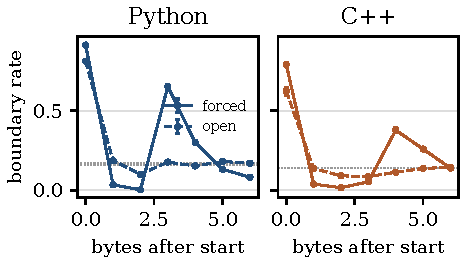
\includegraphics[width=\columnwidth]{generated/p4_offsets.pdf}
\caption{Boundary rate at each byte offset after a constituent start, forced openers (solid) vs.\ open-ended (dashed); dotted line: null rate.}
\label{fig:offsets}
\end{figure}
\xTableArms
\begin{figure*}[t]
\centering
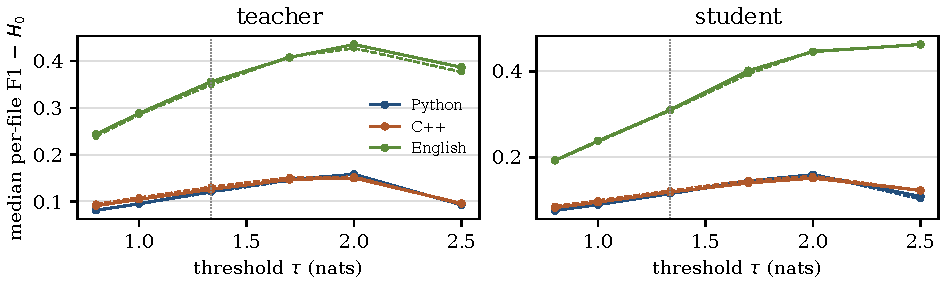
\includegraphics[width=\textwidth]{generated/tau_sweep.pdf}
\caption{Pre-registered threshold sweep on calibration files: median per-file F1 margin over $H_0$ ($k=0$, 10{,}000 permutations). Dotted: the checkpoint's $\tau=1.335$.}
\label{fig:tau}
\end{figure*}
\xTableRatio
\xTableRobust
\xTableK
\TableOFour
\TableIoU
\xTableTfiveTwelve
\xTableEff
\xTableAlpha

\section{Fidelity Gates and Example Segmentation}
\label{app:fidelity}
\begin{table}[h]
\centering\small
\begin{adjustbox}{max width=\columnwidth}
\begin{tabular}{lll}
\toprule
Gate & What it checks & Outcome \\
\midrule
G1 & weights, counts and checksums match provenance & pass \\
G2 & tokenizer emits BOS + byte offsets (EOS criterion mis-specified) & amended \\
G3 & HF logits equal an independent re-implementation ($1.05\times10^{-4}$) & pass \\
G4 & entropy is Shannon entropy in nats & pass \\
G5 & boundary rule equals HF \texttt{patch\_lengths} on 28/28 inputs & pass \\
G6 & influence vanishes beyond the 512-token window & pass \\
G7 & low entropy on repeats, high density on random bytes & amended \\
G8 & reruns are bit-identical & pass \\
\bottomrule
\end{tabular}
\end{adjustbox}
\caption{Checkpoint-fidelity gates (unchanged from the mid-submission).}
\end{table}
The patcher's segmentation of a short Python function, with patch starts marked by \texttt{|}:
\begin{quote}\small\ttfamily
d|e|f |f|i|b|onacci|(|n|):\\
\quad|if n |< |2|:\\
\quad\quad|return |n|\\
\quad|return |fibonacci(n |- 1) |+ |fibonacci(n - 2)
\end{quote}
Boundaries open statements after indentation, and the bytes after \texttt{if} and \texttt{return} stay inside one patch. An identifier is split at nearly every byte on first use and kept whole on reuse.
\begin{figure*}[t]
\centering
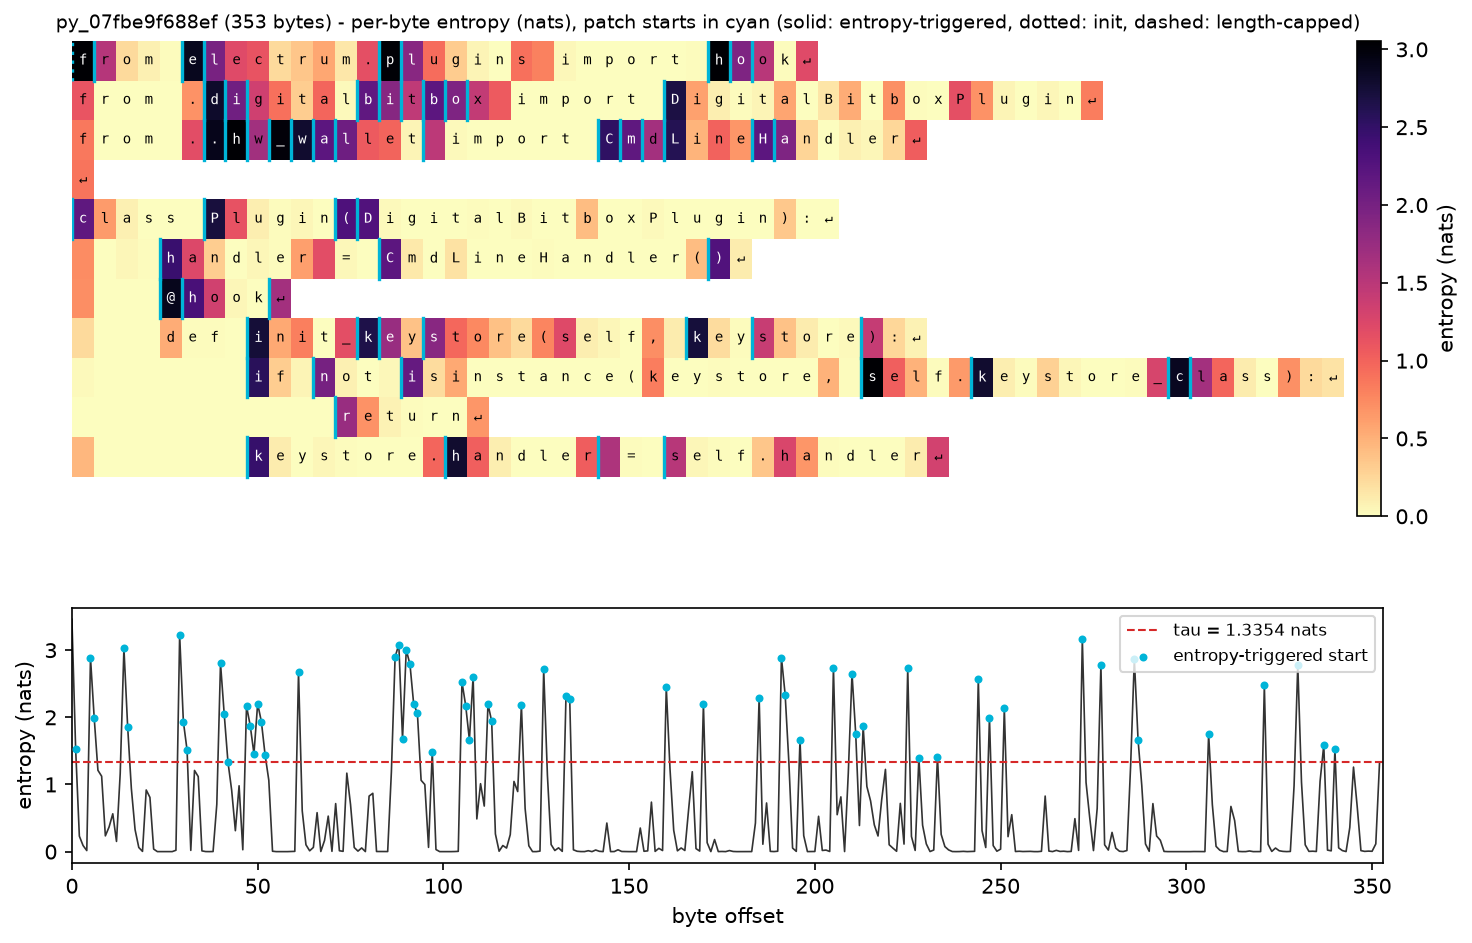
\includegraphics[width=.49\textwidth]{../../results/figures/stream_a/swa512-float32-t1.3354-mplnone-91aa6b8e/entropy_heatmap_py_07fbe9f688ef.png}\hfill
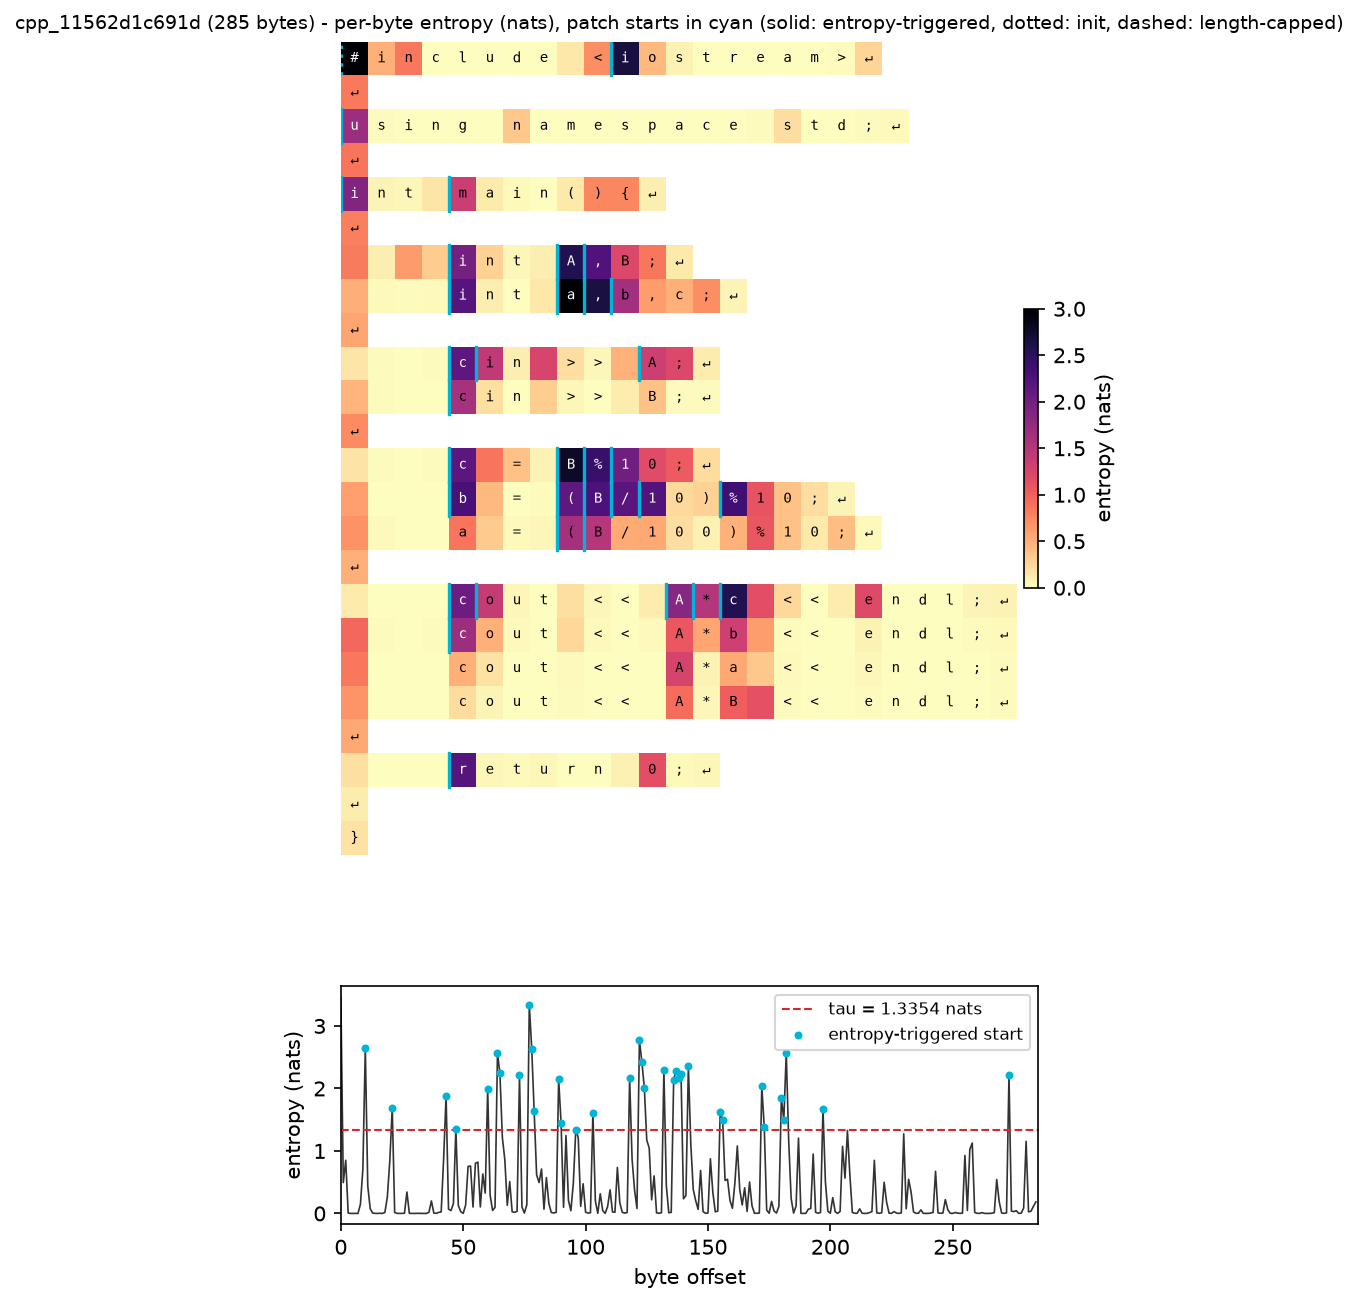
\includegraphics[width=.49\textwidth]{../../results/figures/stream_a/swa512-float32-t1.3354-mplnone-91aa6b8e/entropy_heatmap_cpp_11562d1c691d.png}\\[2pt]
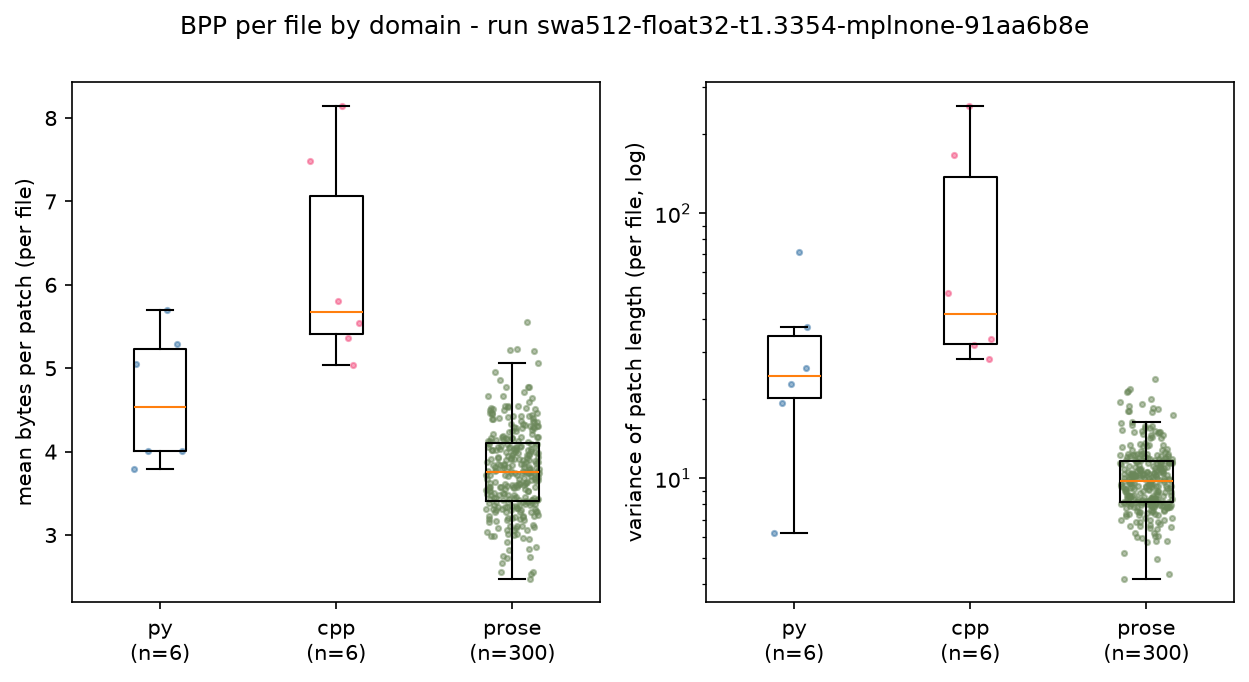
\includegraphics[width=.49\textwidth]{../../results/figures/stream_a/swa512-float32-t1.3354-mplnone-91aa6b8e/bpp_distributions.png}\hfill
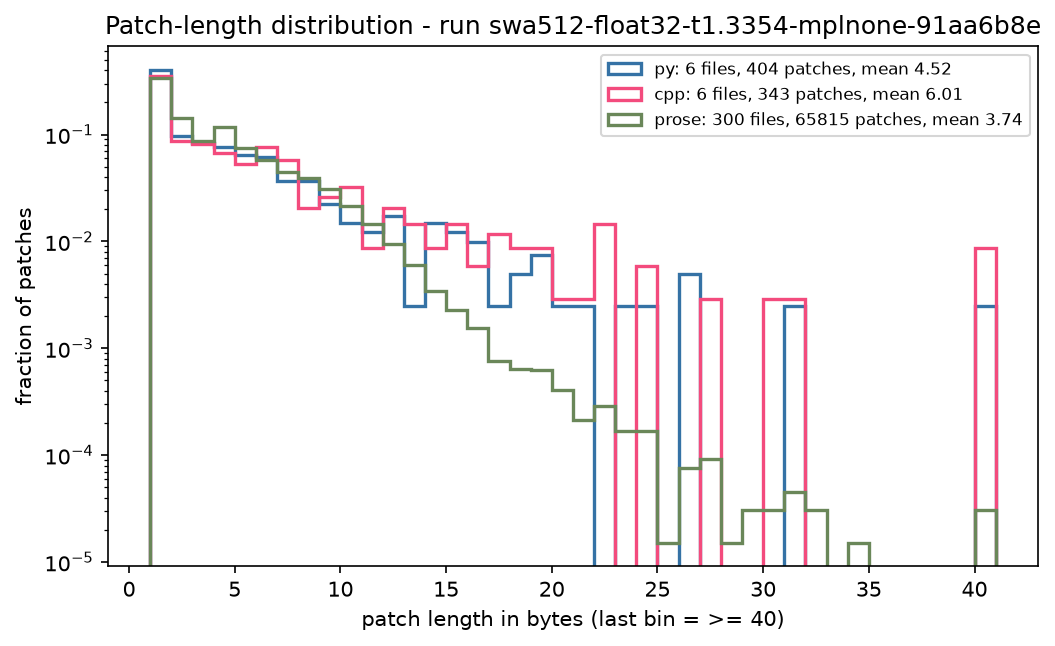
\includegraphics[width=.49\textwidth]{../../results/figures/stream_a/swa512-float32-t1.3354-mplnone-91aa6b8e/patch_length_distribution.png}
\caption{Proposal deliverable (4): per-byte entropy heatmaps for a Python and a C++ file, and BPP and patch-length distributions per language (frozen teacher run).}
\label{fig:heatmaps}
\end{figure*}
